% Created by tikzDevice version 0.7.0 on 2014-09-25 14:00:56
% !TEX encoding = UTF-8 Unicode
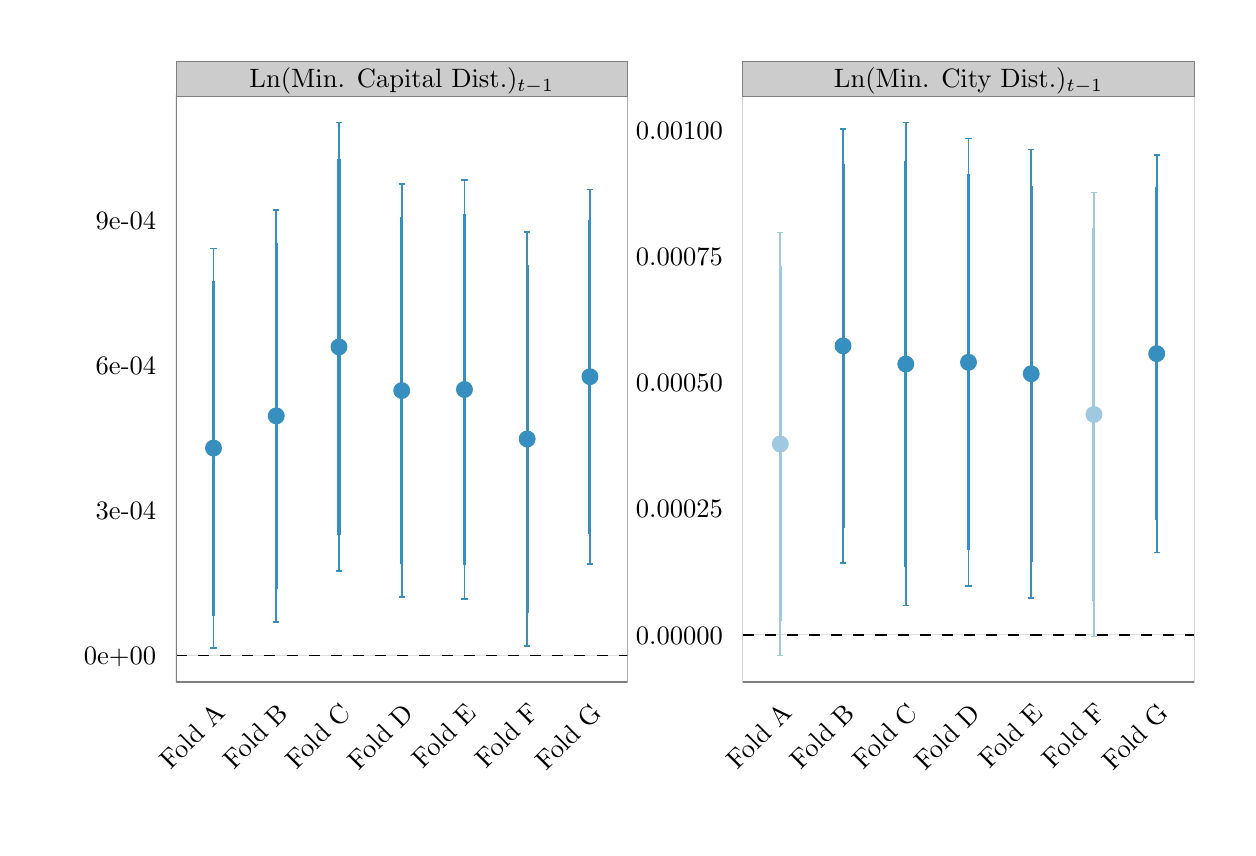
\begin{tikzpicture}[x=1pt,y=1pt]
\definecolor[named]{fillColor}{rgb}{1.00,1.00,1.00}
\path[use as bounding box,fill=fillColor,fill opacity=0.00] (0,0) rectangle (433.62,289.08);
\begin{scope}
\path[clip] (  0.00,  0.00) rectangle (433.62,289.08);
\definecolor[named]{drawColor}{rgb}{1.00,1.00,1.00}
\definecolor[named]{fillColor}{rgb}{1.00,1.00,1.00}

\path[draw=drawColor,line width= 0.6pt,line join=round,line cap=round,fill=fillColor] ( -0.00,  0.00) rectangle (433.62,289.08);
\end{scope}
\begin{scope}
\path[clip] ( 53.55, 52.60) rectangle (216.77,264.40);
\definecolor[named]{fillColor}{rgb}{1.00,1.00,1.00}

\path[fill=fillColor] ( 53.55, 52.60) rectangle (216.77,264.40);
\definecolor[named]{drawColor}{rgb}{0.21,0.56,0.75}
\definecolor[named]{fillColor}{rgb}{0.21,0.56,0.75}

\path[draw=drawColor,draw opacity=0.30,line width= 0.3pt,line join=round,fill=fillColor,fill opacity=0.30] ( 67.15, 65.03) -- ( 67.15,209.31);

\path[draw=drawColor,draw opacity=0.30,line width= 0.3pt,line join=round,fill=fillColor,fill opacity=0.30] ( 89.82, 74.37) -- ( 89.82,223.23);

\path[draw=drawColor,draw opacity=0.30,line width= 0.3pt,line join=round,fill=fillColor,fill opacity=0.30] (112.49, 92.67) -- (112.49,254.77);

\path[draw=drawColor,draw opacity=0.30,line width= 0.3pt,line join=round,fill=fillColor,fill opacity=0.30] (135.16, 83.37) -- (135.16,232.52);

\path[draw=drawColor,draw opacity=0.30,line width= 0.3pt,line join=round,fill=fillColor,fill opacity=0.30] (157.83, 82.70) -- (157.83,233.97);

\path[draw=drawColor,draw opacity=0.30,line width= 0.3pt,line join=round,fill=fillColor,fill opacity=0.30] (180.50, 65.59) -- (180.50,215.32);

\path[draw=drawColor,draw opacity=0.30,line width= 0.3pt,line join=round,fill=fillColor,fill opacity=0.30] (203.17, 95.32) -- (203.17,230.62);
\definecolor[named]{drawColor}{rgb}{0.21,0.56,0.75}
\definecolor[named]{fillColor}{rgb}{0.21,0.56,0.75}

\path[draw=drawColor,line width= 1.1pt,line join=round,fill=fillColor] ( 67.15, 76.63) -- ( 67.15,197.71);

\path[draw=drawColor,line width= 1.1pt,line join=round,fill=fillColor] ( 89.82, 86.34) -- ( 89.82,211.26);

\path[draw=drawColor,line width= 1.1pt,line join=round,fill=fillColor] (112.49,105.70) -- (112.49,241.74);

\path[draw=drawColor,line width= 1.1pt,line join=round,fill=fillColor] (135.16, 95.36) -- (135.16,220.53);

\path[draw=drawColor,line width= 1.1pt,line join=round,fill=fillColor] (157.83, 94.86) -- (157.83,221.81);

\path[draw=drawColor,line width= 1.1pt,line join=round,fill=fillColor] (180.50, 77.62) -- (180.50,203.28);

\path[draw=drawColor,line width= 1.1pt,line join=round,fill=fillColor] (203.17,106.20) -- (203.17,219.75);
\definecolor[named]{drawColor}{rgb}{0.00,0.00,0.00}
\definecolor[named]{fillColor}{rgb}{0.00,0.00,0.00}

\path[draw=drawColor,line width= 0.6pt,dash pattern=on 4pt off 4pt ,line join=round,fill=fillColor] ( 53.55, 62.23) -- (216.77, 62.23);
\definecolor[named]{drawColor}{rgb}{0.21,0.56,0.75}
\definecolor[named]{fillColor}{rgb}{0.21,0.56,0.75}

\path[draw=drawColor,line width= 0.4pt,line join=round,line cap=round,fill=fillColor] ( 67.15,137.17) circle (  2.85);

\path[draw=drawColor,line width= 0.4pt,line join=round,line cap=round,fill=fillColor] ( 89.82,148.80) circle (  2.85);

\path[draw=drawColor,line width= 0.4pt,line join=round,line cap=round,fill=fillColor] (112.49,173.72) circle (  2.85);

\path[draw=drawColor,line width= 0.4pt,line join=round,line cap=round,fill=fillColor] (135.16,157.94) circle (  2.85);

\path[draw=drawColor,line width= 0.4pt,line join=round,line cap=round,fill=fillColor] (157.83,158.33) circle (  2.85);

\path[draw=drawColor,line width= 0.4pt,line join=round,line cap=round,fill=fillColor] (180.50,140.45) circle (  2.85);

\path[draw=drawColor,line width= 0.4pt,line join=round,line cap=round,fill=fillColor] (203.17,162.97) circle (  2.85);

\path[draw=drawColor,line width= 0.6pt,line join=round] ( 66.02,209.31) --
	( 68.29,209.31);

\path[draw=drawColor,line width= 0.6pt,line join=round] ( 67.15,209.31) --
	( 67.15, 65.03);

\path[draw=drawColor,line width= 0.6pt,line join=round] ( 66.02, 65.03) --
	( 68.29, 65.03);

\path[draw=drawColor,line width= 0.6pt,line join=round] ( 88.69,223.23) --
	( 90.95,223.23);

\path[draw=drawColor,line width= 0.6pt,line join=round] ( 89.82,223.23) --
	( 89.82, 74.37);

\path[draw=drawColor,line width= 0.6pt,line join=round] ( 88.69, 74.37) --
	( 90.95, 74.37);

\path[draw=drawColor,line width= 0.6pt,line join=round] (111.36,254.77) --
	(113.62,254.77);

\path[draw=drawColor,line width= 0.6pt,line join=round] (112.49,254.77) --
	(112.49, 92.67);

\path[draw=drawColor,line width= 0.6pt,line join=round] (111.36, 92.67) --
	(113.62, 92.67);

\path[draw=drawColor,line width= 0.6pt,line join=round] (134.03,232.52) --
	(136.29,232.52);

\path[draw=drawColor,line width= 0.6pt,line join=round] (135.16,232.52) --
	(135.16, 83.37);

\path[draw=drawColor,line width= 0.6pt,line join=round] (134.03, 83.37) --
	(136.29, 83.37);

\path[draw=drawColor,line width= 0.6pt,line join=round] (156.70,233.97) --
	(158.96,233.97);

\path[draw=drawColor,line width= 0.6pt,line join=round] (157.83,233.97) --
	(157.83, 82.70);

\path[draw=drawColor,line width= 0.6pt,line join=round] (156.70, 82.70) --
	(158.96, 82.70);

\path[draw=drawColor,line width= 0.6pt,line join=round] (179.37,215.32) --
	(181.63,215.32);

\path[draw=drawColor,line width= 0.6pt,line join=round] (180.50,215.32) --
	(180.50, 65.59);

\path[draw=drawColor,line width= 0.6pt,line join=round] (179.37, 65.59) --
	(181.63, 65.59);

\path[draw=drawColor,line width= 0.6pt,line join=round] (202.04,230.62) --
	(204.30,230.62);

\path[draw=drawColor,line width= 0.6pt,line join=round] (203.17,230.62) --
	(203.17, 95.32);

\path[draw=drawColor,line width= 0.6pt,line join=round] (202.04, 95.32) --
	(204.30, 95.32);
\definecolor[named]{drawColor}{rgb}{0.50,0.50,0.50}

\path[draw=drawColor,line width= 0.6pt,line join=round,line cap=round] ( 53.55, 52.60) rectangle (216.77,264.40);
\end{scope}
\begin{scope}
\path[clip] (258.35, 52.60) rectangle (421.58,264.40);
\definecolor[named]{fillColor}{rgb}{1.00,1.00,1.00}

\path[fill=fillColor] (258.35, 52.60) rectangle (421.57,264.40);
\definecolor[named]{drawColor}{rgb}{0.62,0.79,0.88}
\definecolor[named]{fillColor}{rgb}{0.62,0.79,0.88}

\path[draw=drawColor,draw opacity=0.30,line width= 0.3pt,line join=round,fill=fillColor,fill opacity=0.30] (271.96, 62.23) -- (271.96,215.06);
\definecolor[named]{drawColor}{rgb}{0.21,0.56,0.75}
\definecolor[named]{fillColor}{rgb}{0.21,0.56,0.75}

\path[draw=drawColor,draw opacity=0.30,line width= 0.3pt,line join=round,fill=fillColor,fill opacity=0.30] (294.63, 95.75) -- (294.63,252.44);

\path[draw=drawColor,draw opacity=0.30,line width= 0.3pt,line join=round,fill=fillColor,fill opacity=0.30] (317.30, 80.30) -- (317.30,254.77);

\path[draw=drawColor,draw opacity=0.30,line width= 0.3pt,line join=round,fill=fillColor,fill opacity=0.30] (339.96, 87.24) -- (339.96,249.09);

\path[draw=drawColor,draw opacity=0.30,line width= 0.3pt,line join=round,fill=fillColor,fill opacity=0.30] (362.63, 83.04) -- (362.63,245.02);
\definecolor[named]{drawColor}{rgb}{0.62,0.79,0.88}
\definecolor[named]{fillColor}{rgb}{0.62,0.79,0.88}

\path[draw=drawColor,draw opacity=0.30,line width= 0.3pt,line join=round,fill=fillColor,fill opacity=0.30] (385.30, 69.14) -- (385.30,229.47);
\definecolor[named]{drawColor}{rgb}{0.21,0.56,0.75}
\definecolor[named]{fillColor}{rgb}{0.21,0.56,0.75}

\path[draw=drawColor,draw opacity=0.30,line width= 0.3pt,line join=round,fill=fillColor,fill opacity=0.30] (407.97, 99.45) -- (407.97,243.12);
\definecolor[named]{drawColor}{rgb}{0.62,0.79,0.88}
\definecolor[named]{fillColor}{rgb}{0.62,0.79,0.88}

\path[draw=drawColor,line width= 1.1pt,line join=round,fill=fillColor] (271.96, 74.51) -- (271.96,202.78);
\definecolor[named]{drawColor}{rgb}{0.21,0.56,0.75}
\definecolor[named]{fillColor}{rgb}{0.21,0.56,0.75}

\path[draw=drawColor,line width= 1.1pt,line join=round,fill=fillColor] (294.63,108.35) -- (294.63,239.84);

\path[draw=drawColor,line width= 1.1pt,line join=round,fill=fillColor] (317.30, 94.33) -- (317.30,240.75);

\path[draw=drawColor,line width= 1.1pt,line join=round,fill=fillColor] (339.96,100.25) -- (339.96,236.08);

\path[draw=drawColor,line width= 1.1pt,line join=round,fill=fillColor] (362.63, 96.06) -- (362.63,232.00);
\definecolor[named]{drawColor}{rgb}{0.62,0.79,0.88}
\definecolor[named]{fillColor}{rgb}{0.62,0.79,0.88}

\path[draw=drawColor,line width= 1.1pt,line join=round,fill=fillColor] (385.30, 82.03) -- (385.30,216.58);
\definecolor[named]{drawColor}{rgb}{0.21,0.56,0.75}
\definecolor[named]{fillColor}{rgb}{0.21,0.56,0.75}

\path[draw=drawColor,line width= 1.1pt,line join=round,fill=fillColor] (407.97,111.00) -- (407.97,231.57);
\definecolor[named]{drawColor}{rgb}{0.00,0.00,0.00}
\definecolor[named]{fillColor}{rgb}{0.00,0.00,0.00}

\path[draw=drawColor,line width= 0.6pt,dash pattern=on 4pt off 4pt ,line join=round,fill=fillColor] (258.35, 69.66) -- (421.58, 69.66);
\definecolor[named]{drawColor}{rgb}{0.62,0.79,0.88}
\definecolor[named]{fillColor}{rgb}{0.62,0.79,0.88}

\path[draw=drawColor,line width= 0.4pt,line join=round,line cap=round,fill=fillColor] (271.96,138.64) circle (  2.85);
\definecolor[named]{drawColor}{rgb}{0.21,0.56,0.75}
\definecolor[named]{fillColor}{rgb}{0.21,0.56,0.75}

\path[draw=drawColor,line width= 0.4pt,line join=round,line cap=round,fill=fillColor] (294.63,174.10) circle (  2.85);

\path[draw=drawColor,line width= 0.4pt,line join=round,line cap=round,fill=fillColor] (317.30,167.54) circle (  2.85);

\path[draw=drawColor,line width= 0.4pt,line join=round,line cap=round,fill=fillColor] (339.96,168.16) circle (  2.85);

\path[draw=drawColor,line width= 0.4pt,line join=round,line cap=round,fill=fillColor] (362.63,164.03) circle (  2.85);
\definecolor[named]{drawColor}{rgb}{0.62,0.79,0.88}
\definecolor[named]{fillColor}{rgb}{0.62,0.79,0.88}

\path[draw=drawColor,line width= 0.4pt,line join=round,line cap=round,fill=fillColor] (385.30,149.31) circle (  2.85);
\definecolor[named]{drawColor}{rgb}{0.21,0.56,0.75}
\definecolor[named]{fillColor}{rgb}{0.21,0.56,0.75}

\path[draw=drawColor,line width= 0.4pt,line join=round,line cap=round,fill=fillColor] (407.97,171.29) circle (  2.85);
\definecolor[named]{drawColor}{rgb}{0.62,0.79,0.88}

\path[draw=drawColor,line width= 0.6pt,line join=round] (270.82,215.06) --
	(273.09,215.06);

\path[draw=drawColor,line width= 0.6pt,line join=round] (271.96,215.06) --
	(271.96, 62.23);

\path[draw=drawColor,line width= 0.6pt,line join=round] (270.82, 62.23) --
	(273.09, 62.23);
\definecolor[named]{drawColor}{rgb}{0.21,0.56,0.75}

\path[draw=drawColor,line width= 0.6pt,line join=round] (293.49,252.44) --
	(295.76,252.44);

\path[draw=drawColor,line width= 0.6pt,line join=round] (294.63,252.44) --
	(294.63, 95.75);

\path[draw=drawColor,line width= 0.6pt,line join=round] (293.49, 95.75) --
	(295.76, 95.75);

\path[draw=drawColor,line width= 0.6pt,line join=round] (316.16,254.77) --
	(318.43,254.77);

\path[draw=drawColor,line width= 0.6pt,line join=round] (317.30,254.77) --
	(317.30, 80.30);

\path[draw=drawColor,line width= 0.6pt,line join=round] (316.16, 80.30) --
	(318.43, 80.30);

\path[draw=drawColor,line width= 0.6pt,line join=round] (338.83,249.09) --
	(341.10,249.09);

\path[draw=drawColor,line width= 0.6pt,line join=round] (339.96,249.09) --
	(339.96, 87.24);

\path[draw=drawColor,line width= 0.6pt,line join=round] (338.83, 87.24) --
	(341.10, 87.24);

\path[draw=drawColor,line width= 0.6pt,line join=round] (361.50,245.02) --
	(363.77,245.02);

\path[draw=drawColor,line width= 0.6pt,line join=round] (362.63,245.02) --
	(362.63, 83.04);

\path[draw=drawColor,line width= 0.6pt,line join=round] (361.50, 83.04) --
	(363.77, 83.04);
\definecolor[named]{drawColor}{rgb}{0.62,0.79,0.88}

\path[draw=drawColor,line width= 0.6pt,line join=round] (384.17,229.47) --
	(386.44,229.47);

\path[draw=drawColor,line width= 0.6pt,line join=round] (385.30,229.47) --
	(385.30, 69.14);

\path[draw=drawColor,line width= 0.6pt,line join=round] (384.17, 69.14) --
	(386.44, 69.14);
\definecolor[named]{drawColor}{rgb}{0.21,0.56,0.75}

\path[draw=drawColor,line width= 0.6pt,line join=round] (406.84,243.12) --
	(409.11,243.12);

\path[draw=drawColor,line width= 0.6pt,line join=round] (407.97,243.12) --
	(407.97, 99.45);

\path[draw=drawColor,line width= 0.6pt,line join=round] (406.84, 99.45) --
	(409.11, 99.45);
\definecolor[named]{drawColor}{rgb}{0.50,0.50,0.50}

\path[draw=drawColor,line width= 0.6pt,line join=round,line cap=round] (258.35, 52.60) rectangle (421.57,264.40);
\end{scope}
\begin{scope}
\path[clip] (  0.00,  0.00) rectangle (433.62,289.08);
\definecolor[named]{drawColor}{rgb}{0.50,0.50,0.50}
\definecolor[named]{fillColor}{rgb}{0.80,0.80,0.80}

\path[draw=drawColor,line width= 0.2pt,line join=round,line cap=round,fill=fillColor] ( 53.55,264.40) rectangle (216.77,277.04);
\definecolor[named]{drawColor}{rgb}{0.00,0.00,0.00}

\node[text=drawColor,anchor=base,inner sep=0pt, outer sep=0pt, scale=  0.96] at (135.16,267.41) {Ln(Min. Capital Dist.)$_{t-1}$};
\end{scope}
\begin{scope}
\path[clip] (  0.00,  0.00) rectangle (433.62,289.08);
\definecolor[named]{drawColor}{rgb}{0.50,0.50,0.50}
\definecolor[named]{fillColor}{rgb}{0.80,0.80,0.80}

\path[draw=drawColor,line width= 0.2pt,line join=round,line cap=round,fill=fillColor] (258.35,264.40) rectangle (421.57,277.04);
\definecolor[named]{drawColor}{rgb}{0.00,0.00,0.00}

\node[text=drawColor,anchor=base,inner sep=0pt, outer sep=0pt, scale=  0.96] at (339.96,267.41) {Ln(Min. City Dist.)$_{t-1}$};
\end{scope}
\begin{scope}
\path[clip] (  0.00,  0.00) rectangle (433.62,289.08);
\definecolor[named]{drawColor}{rgb}{0.00,0.00,0.00}

\node[text=drawColor,anchor=base east,inner sep=0pt, outer sep=0pt, scale=  0.96] at ( 46.44, 58.92) {0e+00};

\node[text=drawColor,anchor=base east,inner sep=0pt, outer sep=0pt, scale=  0.96] at ( 46.44,111.38) {3e-04};

\node[text=drawColor,anchor=base east,inner sep=0pt, outer sep=0pt, scale=  0.96] at ( 46.44,163.84) {6e-04};

\node[text=drawColor,anchor=base east,inner sep=0pt, outer sep=0pt, scale=  0.96] at ( 46.44,216.30) {9e-04};
\end{scope}
\begin{scope}
\path[clip] (  0.00,  0.00) rectangle (433.62,289.08);
\definecolor[named]{drawColor}{rgb}{0.00,0.00,0.00}

\node[text=drawColor,anchor=base east,inner sep=0pt, outer sep=0pt, scale=  0.96] at (251.24, 66.35) {0.00000};

\node[text=drawColor,anchor=base east,inner sep=0pt, outer sep=0pt, scale=  0.96] at (251.24,111.91) {0.00025};

\node[text=drawColor,anchor=base east,inner sep=0pt, outer sep=0pt, scale=  0.96] at (251.24,157.46) {0.00050};

\node[text=drawColor,anchor=base east,inner sep=0pt, outer sep=0pt, scale=  0.96] at (251.24,203.02) {0.00075};

\node[text=drawColor,anchor=base east,inner sep=0pt, outer sep=0pt, scale=  0.96] at (251.24,248.58) {0.00100};
\end{scope}
\begin{scope}
\path[clip] (  0.00,  0.00) rectangle (433.62,289.08);
\definecolor[named]{drawColor}{rgb}{0.00,0.00,0.00}

\node[text=drawColor,rotate= 45.00,anchor=base east,inner sep=0pt, outer sep=0pt, scale=  0.96] at ( 71.83, 40.81) {Fold A};

\node[text=drawColor,rotate= 45.00,anchor=base east,inner sep=0pt, outer sep=0pt, scale=  0.96] at ( 94.50, 40.81) {Fold B};

\node[text=drawColor,rotate= 45.00,anchor=base east,inner sep=0pt, outer sep=0pt, scale=  0.96] at (117.17, 40.81) {Fold C};

\node[text=drawColor,rotate= 45.00,anchor=base east,inner sep=0pt, outer sep=0pt, scale=  0.96] at (139.84, 40.81) {Fold D};

\node[text=drawColor,rotate= 45.00,anchor=base east,inner sep=0pt, outer sep=0pt, scale=  0.96] at (162.51, 40.81) {Fold E};

\node[text=drawColor,rotate= 45.00,anchor=base east,inner sep=0pt, outer sep=0pt, scale=  0.96] at (185.17, 40.81) {Fold F};

\node[text=drawColor,rotate= 45.00,anchor=base east,inner sep=0pt, outer sep=0pt, scale=  0.96] at (207.84, 40.81) {Fold G};
\end{scope}
\begin{scope}
\path[clip] (  0.00,  0.00) rectangle (433.62,289.08);
\definecolor[named]{drawColor}{rgb}{0.00,0.00,0.00}

\node[text=drawColor,rotate= 45.00,anchor=base east,inner sep=0pt, outer sep=0pt, scale=  0.96] at (276.63, 40.81) {Fold A};

\node[text=drawColor,rotate= 45.00,anchor=base east,inner sep=0pt, outer sep=0pt, scale=  0.96] at (299.30, 40.81) {Fold B};

\node[text=drawColor,rotate= 45.00,anchor=base east,inner sep=0pt, outer sep=0pt, scale=  0.96] at (321.97, 40.81) {Fold C};

\node[text=drawColor,rotate= 45.00,anchor=base east,inner sep=0pt, outer sep=0pt, scale=  0.96] at (344.64, 40.81) {Fold D};

\node[text=drawColor,rotate= 45.00,anchor=base east,inner sep=0pt, outer sep=0pt, scale=  0.96] at (367.31, 40.81) {Fold E};

\node[text=drawColor,rotate= 45.00,anchor=base east,inner sep=0pt, outer sep=0pt, scale=  0.96] at (389.98, 40.81) {Fold F};

\node[text=drawColor,rotate= 45.00,anchor=base east,inner sep=0pt, outer sep=0pt, scale=  0.96] at (412.65, 40.81) {Fold G};
\end{scope}
\end{tikzpicture}
